%%%%%%%%%%%%%%%%%%%%%%%%%%%%%%%%%%%%%%%%%%%%%%%%%%%%%%%%%%%
%%%%%%%%%%%%%%%%%%%%%%%%%%%%%%%%%%%%%%%%%%%%%%%%%%%%%%%%%%%
\subsection{XRD}
\begin{figure}
	\centering
	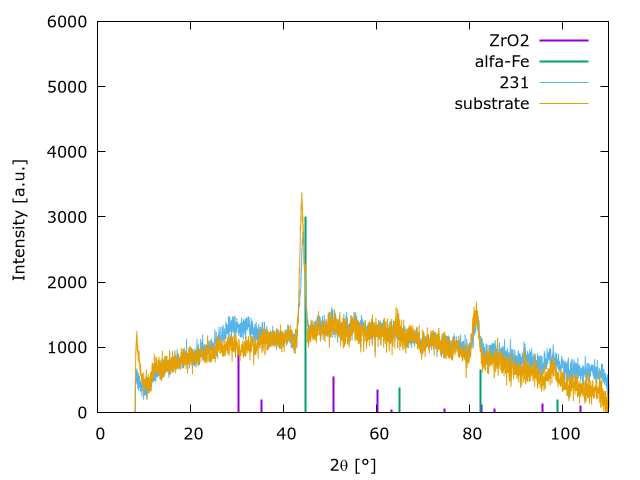
\includegraphics[width=\picwidth]{Pics/xrd.png}
	\caption{XRD spectra}
	\label{fig:xrd}
\end{figure}

%%%%%%%%%%%%%%%%%%%%%%%%%%%%%%%%%%%%%%%%%%%%%%%%%%%%%%%%%%%
%%%%%%%%%%%%%%%%%%%%%%%%%%%%%%%%%%%%%%%%%%%%%%%%%%%%%%%%%%%
\subsection{SEM}

%%%%%%%%%%%%%%%%%%%%%%%%%%%%%%%%%%%%%%%%%%%%%%%%%%%%%%%%%%%
%%%%%%%%%%%%%%%%%%%%%%%%%%%%%%%%%%%%%%%%%%%%%%%%%%%%%%%%%%%
\subsection{V-I and PSO//Optimization}
\td{ideal objective is to create response surface approximation}\\
\td{the input vars were not regularized/normalized, naively like a small child eating old food and regretting not informing oneself earlier}\\
\td{too much data as input, dimensionality reduction (PCA) and optimization}\\
\td{plot the predicted data for variables which should be excluded (Tcal, Vcal,Conc, layers)}
\td{pre optimization was used to check if limits where okay, but could also have been used to sieve out factors without impact on response (see miller 2001 \cite{miller2001using} section 1) }
The primary goal of a screening experiment is to identify the active factors. 
A secondary goal is to provide a simple model that captures the essential features of the 
relationship between these active factors and the response—that is, to identify the active effects. \cite{miller2001using}

\td{show results between 1ml acoh (199), acoh+ipo 1:1 (201) and ipo (192). Show graph of the three vs log pondus G and pinhole density and maybe distribution of single point measurements? 
\texttt{set boxwidth 2; set xtics 5; p "stat.dat" u 1:3 with boxes} 
}

\td{base/best sample was somewhot 150, 5 layers 3F 2K/min 400C} what was the best result?
\td{
double calcination (2x400C) was tried instead of pyrolization (4x200 then 400C),p49
so higher concentration of zro2 leads to less stable solution
5F ca 100min
4F ca 140min
3F ca 420min (7h)
}
\td{if i would plan the optimisation again, I would take less input variables (fokus on 
conc,vdoc and tdoc or even only vdoc and tdoc) which may or may not have multiple maxima.}
\td{adding a extra variable to optimize was to optimistic and ich hab mir damit eindeutig 
(im nachhinein) steine in den Weg gelegt.}
\td{instead of changing the stabilisation agent before optimisation, could change after pso}
\td{varied doctor blading velocity: 10, 5, 1, 0.5, 0.2, 0.1. Slower less layer}
\todo{Following stirring times (in minutes) were tested and didn't have an influence on stability of the solution: 10-10-20, 10-10-45, 30-30-180.}
The space seems to be too big for the small sample size.
Look at relation of space size and sample size here and in Hu2016.
\td{p68 iPrOH to milky solution and solution becomes clear!!!! checked how much 
is needed. 5F solution milky over night ~2ml, added 1ml IPO and clear.}
\td{extra PB-design with conc(2-4), layers(6-8), tcal(430-470), tvel(4-6),
vdoc(0.5-2), tdoc(40-60). low vdoc very homogenuous but actually nearly no 
deposition because miniscus is pulling liquid off the substrate.}
\td{IPO influence on "stability" p74: 600ul IPO makes clear, 4000 ul BuOH not clear with 
same base solution (1ml of 4F), added extra 400ul to BuOH sol and after 5min clear. 
of 1:5 is unacceptable Dilution }
21.8 (1F) from 15.02. 13:30 bis 
26.3 (1ml iPO to ca2ml of 5f) from 16.02. 16:30 bis 18.02.++
18.02 4F in 80min milky
      2F in ca 24h (stabilization AcOH)
\td{In example of documentation 2 input variables and 1-2 responses initial population=10
, subsequent population=5, but 10 iterations. Clearly more input varibles and less 
iterations (as in actual experiments) lead to suboptimal results.
When plotting input vars  against the response variables, no trend
The exploration-vs-exploitation parameters of the model were also not set accordingly.}
see \href{https://search.r-project.org/CRAN/refmans/emma/html/emma.html}{source}


Would be easier to fit with single factor at a time variation or latin hyper cuber?
Would it also be easier for PSO or ML to find fitting function?
Every output var is independent of each other, so $v_{cal}$ can act as test 

plot predictions from EMMA and ML.
the data has a lot of error, but because the production process takes so long nad the limited time and the chosen optimisation method, the experiments weren't weiderholt
how much variance is in data? 

The most time consuming part was definitively the prelaminary studies.
this time could have been verkürzt by testing a wide array of diverse recipes from the literature

The data is spread across the datenraum, such that it is not trivial to (1) find the variable with the most variance and (2) to fit in order to understand to impact of noise on the data. 
Dimension reduction bietet sich stark an bei solcher Datenlage. 
Welche methode funktioniert bei relativ vielen variablen, wenig datenpunkten und Noise. 
Am besten waere feature extraction (variable x1 hat am meisten einfluss. ginge auch wenn man bei pca den einfluss von verschiedenen 

heating rate was one of the dependent variables with the intention of minimizing the variable. 
It can also be used as test to see how well the GA performes
It doesn't influence the fit for the other splines, but it influences the choice of samples therefore it might have slowed down the process
Overall there were too many variables involved for such a small dataset

first recipe tried to improve to achieve more restisting layer. by pH value, surface 
tensionand solution ratios (only 10\% change because it was assumed, that the recipe is 
good and should be improved, but the recipe should be altered thoroughly.
two layers were also tried but didn't even pass the visual examination/test/inspection. 
A curst was produced. 
At this point in time everything was doctor bladed by hand. The hight was varied (with tape).
When the switch to the erichsen was made. The height was kept constant in order to keep 
the variables to optimize ueberschuabar, but could have been even less variables.
If the movement was to slow the resluting  layer would be very inhomogenuous, thus the
velocity wasn't varied.

aquatic vs buthanolic
aquatic immidiately milky

\td{p75 tested various vDOC (10,15,20) with TDOC (40,60,70,80) variations with only visual 
inspection of evaporation process. Ideally solution evaporate shortly after DB but not 
before} 
n-BuOH has boiling point of ca 117C 
\href{https://pubchem.ncbi.nlm.nih.gov/compound/1-butanol#section=Boiling-Point}{source}
\td{p74 146,150,151,152,153,154,156,157,158,160,161,186,187,188,190,194,195,198 
all sputtered with Ag silver on 19.02.2021.}
EMMA was finished on 23.02.2021
first experiments generated, but trashed because 1F solution neglected, contraints 
tightened
p76, 146 (10x1F) good, 154 (3x4F) okay, 156 (3x3F) bad visualisation
look at visualisation in code/pca/ folder and maybe use sort -n 3 
which values were actually used in EMMA and how were they calculated
from 145 to 160 what was changed, large increase of G
small better!!!
p82 test to what extend AcOH can be replaced with iPOH
192 was first with IPOH
use Kernel ridge regression, in PSO the distance of response variables is 
preparation before measuring the i-v: removing layer by scratching in order to to the 
steel subtrate. measure resistance if very low (around 10-1) apply paste and let dry
why different output with ptyhon 3.6 (work laptop) and 3.8 personal
discussion: 
why is IPO satbilizing? 
what are reasons for instability? 
IV aufbau p 103 
TODO: check which software versions
check if output of 
check if outputs provided by all-stat.sh is same as in R  (p 100)
look at last pages of notebook
\td{maybe the observable/sumofsquareddistanceoflogofconductance is not a good metric.
I should have a look at the raw data. maybe try to verarbeiten different and then fit 
with KRR or SVM, is phd a sigmoid function? }

\td{for 1F c(Zr) = 44.6 mmol/L
if n is number of samples, and p is number of input variables, then n >> p 
In this case n\~50 and p\~6 which give n/p=8+1/3
in EMMA documentation example n=55and p=1-2, n/p=55-22.5
plot x vs G and hold all other vars const
write script to do that}

\todo{make sample time line with ipo vs acoh, al vs ag, hg vs doc, ...}

\td{
acceptable layer was produced by buthanolic solution, but very unstable (short lived) how long? p41 
extra AcOH stabilzed but needed so much that dilution too large...
The stirring time was untersucht, but not much difference so shortest was used because 
short time can produces faster and the resulting solution is longer stable 
(after finishing mixing)
10 layers were tried of short stiring and gave good results? samples 130,131,134,135 (p43)
}

\td{longer literature research (first solution,second solution) and PSO wrongly eingeschaetzt, 
could have been verhindert durch lesen the docu and more papers more thoughoughly. 
Ich war geblendet von dem was ich wollte und dadurch nicht realistisch}
%\td{I-V: 2 terminal measurement one terminal was varibale and the other the ground from $-5*10^{-3}$ V to $5*10^{-3}$ V with steps of $10^{-2}$ measure current from back bone to backbone if shorted, then can measure actual resistance of layer. resistance of steel is neglectable. In order to get an impression of the quality of the layer mutliple contact (picture) are sputtered (throuhg a mask) and statistics: Two angabewerte: the weighted durchschnit and the number of pinholes, ie the number of contacts which were shorted, have an resistance below an threshold. if tunneling, iv follows powerlaw, if direct contact, iv follows linear }
\td{I wanted to exhaust the possibilities of EA (not having enough data). i should have rather einengen the search raum as much as possible (spreading the search room too much) and then do optimisation: fix layer count to 3 fix conc to 3F and fix calc temp and rate (or only use two extreme values)}

\td{I wanted to let the algorithm show what I already knew instead of letting my a priori knowledge constrain the model before starting.}

\subsection{DOE}
factorial design (classical \gls{doe} is more robust at feature extraction for error laden data \cite{giunta2003overview}

\td{"Similarly, it is often wise not to plan a comprehensive experiment that involves a large number of factors of interest. Such an experiment presupposes that most or all of the factors are important contributors to changes in the response variable and that they contribute jointly; i.e., that individual factor effects and their interactions are statistically significant and meaningful." - from Gunst2007 
but on the other hand 
If one ain't sure a if factor is relevant, the model should be able to detect if there is a influence. - from Haertler2014?

let's rule out different input variables: \\
does the heating temperature influence the resistance?  no \\
does the heating velocity influence the resistance?  hardly\\
do conc and layers number influence resistance? linear \\
do db velocity and db temperautre influence resistance? how\\

somebody very wise (my superviser) once said: we need to able to predict it otherwise it is just an engineering problem \td{(look at mail)}

"Je grösser nämlich die Anzahl freier Parameter im Modell ist, umso grösser ist der erforderliche Datenumfang und umso ungenauer wir die statistisch gewonnene Aussgae bei gleichem Datenumfang." - Gisela Härtler\cite{haertler2014statistisch}

\td{make analysis with EMMA dataset and EMMA+DOE}
\td{talk about the switch of recipe before emma: makes experiments hard/impossible to compare, but more practical and proof that it works weell} 

\td{The disadvantage of ANOVA is that information is lost because independent variables are assumed categorical even though they are ordinal}

% https://journals-sagepub-com.uaccess.univie.ac.at/doi/pdf/10.1177/0013164495055004001
% https://www.researchgate.net/profile/Barbara-Tabachnick/publication/259465542_Experimental_Designs_Using_ANOVA/links/5e6bb05f92851c6ba70085db/Experimental-Designs-Using-ANOVA.pdf
% https://stats.stackexchange.com/questions/137631/is-it-appropriate-to-do-an-anova-on-a-feature-selected-via-inspecting-pca-result
% https://link.springer.com/chapter/10.1007/978-3-642-32639-4_15

plot generation against conductivity

comparison of size: 
see Notes/ga_from_lit_summary.txt 
what is the minimum of population*generation and what is 10*5 


